% {Youssouph Cissokho}
\newpage
\  
\newpage
\section{Anomalies et données de grande dimension}
%
One se réfère principalement dans cette section  à Aggarwal (2017) \cite{A1}, Aggarwal et Sathe (2017) \cite{A8}, Ranga et al. (2019) \cite{A10} and Lazarevic et al.(2005) \cite{A14} .\newl 
La détection des valeurs aberrantes est un vaste domaine qui a été étudié dans le cadre d’un grand nombre de domaines d’application. De nos jours, de nombreuses données réelles sont de très grandes dimensions, dans certains scénarios, les données peuvent contenir \textbf{des centaines ou des milliers de dimensions}. De nombreux algorithmes récents utilisent des concepts de proximité (distances) afin de déterminer les valeurs aberrantes en fonction de leur relation avec le reste des données.  Cependant,  en haute dimension l’espace les données se retrouvent  isolées et deviennent éparses et la notion de proximité ne parvient pas à conserver son importance. En conséquence, pour les données de grande dimension, la notion de définition de valeurs aberrantes significatives est beaucoup plus complexe et non évidente.  Ainsi, beaucoup de  méthodes conventionnelles de  détection des valeurs aberrantes ne fonctionnent pas très efficacement, \textbf{ceci est un artefact connu sous le nom de  la malédiction ou fléau de la dimensionalité}. \newl
Le reste de cette section est organisé comme suit: dans un premier temps, une tentative de définition est donnée ainsi que les défis, ensuite, on étudiera les techniques de détection des valeurs aberrantes et enfin, on présentera la méthode des ensembles ainsi que celle des sous-espaces. 
%
%
\subsection{Definition and défis}
%
%
Une valeur aberrante est une observation qui s'écarte ou a des comportements différents des autres observations dans la donnée qui suscite les soupçons qu'elle a été générée par un autre
mécanisme. Les valeurs aberrantes sont également appelées anomalies, discordants, déviants,
dans la littérature relative à l'exploration de données et aux statistiques. \cite{A1}\newl
La difficulté de la détection des valeurs aberrantes ou anomalies en grande dimension réside dans le fait que la notion de distance ne parvient pas à conserver son importance on parle ainsi du fléau de la dimensionalité. C'est en ce sens qu'il est dit que le problème détection des valeurs aberrantes est comme trouver une aiguille dans une botte de foin \cite{A14}
%
\subsection{Méthode de réduction de la dimension: ACP, DOBIN}
%
Comme mentionné ci-haut, on a des données de très grande dimension, lesquelles peuvent contenir des centaines de dimensions et cela à pour conséquence  que les méthodes conventionnelles de  détection des anomalies ou valeurs aberrantes ne fonctionnent pas très efficacement. Pour contrer ce problème, une des solutions consiste à réduire la dimension, tout en gardant l'essentiel des caractéristiques des données. C'est la réduction de la dimensionnalité. On peut citer entre autres,\textbf{ analyse en composantes principales,  analyse discriminante linéaire, sélection de caractéristique etc}. Deux approches classiques sont \textbf{la sélection des caractéristiques}, qui consiste à choisir un petit ensemble de variables représentatives des observations, et \textbf{analyse en composantes principales} feront l'objet d'une étude détaillée pour la suite.
%
\subsubsection*{Analyse en composantes principales(ACP)}
%
L'ACP cherche à trouver une représentation dans l’espace de dimension inférieure (projeter les points sur une droite, un plan, ...un sous-espace ) des données contenant la plus grande variation possible. Elle correspond donc à une  transformation linéaire orthogonale transformant les données en un nouveau système de coordonnées, de sorte que la plus grande variance résultant d’une projection scalaire des données se situe sur la première coordonnée (appelée première composante principale), la deuxième plus grande variance sur la seconde coordonnée, etc. \newl
Étant donné une matrice des données $n\times p$, $\textbf{X}=(X_1,\cdots,X_p)$ à $n$ observations (nombre de lignes) et $p$ variables (nombre de colonnes) centrée et réduite. Les composantes principales, qui sont une combinaisons linéaires des variables, sont données par les variables  suivantes
\begin{align*}
\textbf{Y}_i=\ell^t_i\textbf{X}=\ell_{1i}\textbf{X},\cdots,\ell_{pi}\textbf{X};\quad i=1,\cdots,k.
\end{align*}
avec ($k\leq p$), qui fournit la plus grande variance sujet à la contrainte $\|\ell_i\|=1$ (ou $\|\cdot\| $ est la norme). 
On en déduit donc
\begin{align*}
\operatorname{var}\left(Y_{i}\right) &=\operatorname{var}\left(\ell_{i}^{t} \boldsymbol{X}\right)=\ell_{i}^{t} \boldsymbol{\Sigma} \ell_{i} \,,\\ 
\operatorname{cov}\left(Y_{i}, Y_{k}\right) &=\operatorname{cov}\left(\ell_{i}^{t} \boldsymbol{X}, \ell_{k}^{t} \boldsymbol{X}\right)=\ell_{i}^{t} \boldsymbol{\Sigma} \ell_{k}\, .
\end{align*}
En d'autres termes,  il faut 
trouver le vecteur $\ell_{i}$ qui  maximise la variance de $Y_i$  ie 
\begin{align*}
\mathbf{\ell}_{1}&=\underset{\|\mathbf{\ell_1}\|=1}{\arg \max }\left\{\ell^t_1\mathbf{X}^{t} \mathbf{X} \ell_1\right\},
\end{align*}
et $\ell_2$ tel que la variance soit maximale et décorrélé avec $\ell_1$,   
\begin{align*}
\mathbf{\ell}_{2}& =\underset{\|\mathbf{\ell_2}\|=1,\;\ell_{1}^{t}\ell_{2} =0}{\arg \max }\left\{\ell^t_2\mathbf{X}^{t} \mathbf{X} \ell_2\right\}.
\end{align*}
De façon similaire, on trouve $\ell_k$ tel que la variance soit maximale et décorrélé avec tous les $\ell_i$, $i<k$ ie
\begin{align}
\mathbf{\ell}_k=\underset{\substack{\|\ell_k\|=1,\\ \;\ell_{i}^{t}\ell_k=0,\;\forall\;i<k}}{\arg \max} \left\{\ell^t_k\mathbf{X}^t \mathbf{X} \ell_k\right\}.\label{eq1}
\end{align}
Pour résoudre \eqref{eq1},  for all $\;i<k$, on utilise le Lagrangien qui  est donné par 
\begin{align*}
L=\ell^t_k\mathbf{X}^t \mathbf{X} \ell_k-\lambda_k(\ell^t_k\ell_k-1)-w\ell_{i}^{t}\ell_k.
\end{align*}
Dérivant le Lagrangien par rapport à chacune des composantes du vecteurs $\ell_k$, $\lambda_k$ et $w$ simplifiant, on trouve: 
\begin{align}
\mathbf{X}^t \mathbf{X} \ell_k&=\lambda_k\ell_k\\
\ell^t_k\ell_k&=1,\; \text{and}\; \ell^t_k\ell_i=0,\;\text{for all}\; i<k.
\end{align}
Le vecteur $\ell_k$ recherché correspond au vecteur propre associé à la $k$ ième plus grande  valeur propre de la matrice $\mathbf{X}^t \mathbf{X}$. D'où le résultat suivant:\

\begin{theorem}
Les $k$ ($k<p$) composantes principales donnant la plus grande variance maximale sont données par les $k$ vecteurs propres associés aux $k$ plus grandes valeurs propres de $\mathbf{X}^t \mathbf{X}$.
\end{theorem}
L'ACP peut être utilisé comme méthode de détection des valeurs aberrantes ou être utilisé comme méthode préalable (réduction de la dimension)  pour un autre  algorithme.  Par ailleurs, elle permet aussi une visualisation en 2 ou 3 dimensions, là ou on ne pouvait pas le faire avec une dimension supéri\newl
\textbf{La proportion de variance expliquée}, on note que 
\begin{align*}
\sum_{i=1}^{k}\operatorname{var}\left(Y_{i}\right) &=\sum_{i=1}^{k}\ell_{i}^{t} \boldsymbol{\Sigma} \ell_{i}=\sum_{i=1}^{k}\lambda_i \,.
\end{align*}
Ainsi, la variance totale de la population est égale à la somme des valeurs propres. Par conséquent, la proportion de la variance totale expliquée par la i ème composante principale est 
\begin{align*}
0\leq \frac{\lambda_i}{\sum_{i=1}^{p}\lambda_i }\leq 1
\end{align*}
\textbf{Combien de composantes principales à retenir}, 
La qualité des résultats de l'ACP dépend fortement du nombres de composantes principales retenues, autrement dit, la dimension  $k$ du sous-espace. Il existe plusieurs méthodes qui traitent ce problème, on présentera juste deux ici: \textbf{la part de variance totale expliquée par les $k$ premier axes principaux} et \textbf{la méthode de l'éboulis}.\\
\textbf{La part de variance totale expliquée par les $k$ premier axes principaux}, est donnée par 
\begin{align*}
p_k=\frac{\sum_{i=1}^{k} \lambda_i}{\sum_{i=1}^{p}\lambda_i }
\end{align*}
On retient donc les $k$ composantes principales de sorte $p_k$  soit supérieure à une valeur prédéfinie (souvent elle est  comprise entre $80\%$ et $90\%$). \newl
\textbf{la méthode de l'éboulis}, consiste à tracer la courbe des valeurs propres de façon décroissante. Le principe consiste à repérer, s'il existe, un "coude" dans le graphe et de ne conserver que les valeurs propres jusqu'à ce coude.
\begin{example}
Un exemple appliqué sur  les \href{1http://web.stanford.edu/ hastie/CASIles/DATA/leukemia big.csv}{donnèes} de mesures de l'expression génique chez 72 patients atteints de leucémie. Il se compose de 7128 gènes. Voir Figure \ref{fig0}.
\begin{figure*}[t]
    \centering
     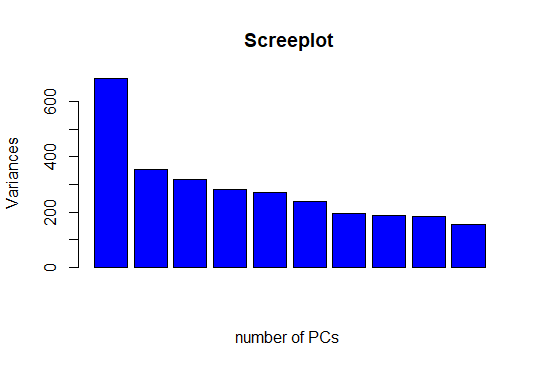
\includegraphics[width=.5\textwidth]{ADOA/Images/screeleuk.png}
    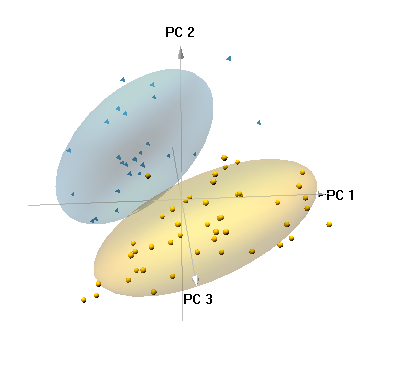
\includegraphics[width=.4\textwidth]{ADOA/Images/3dpcleuk.PNG}
    \caption{Courbe d'éboulis (gauche), projection des données sur 3 composantes (droite)}\hrule
    \label{fig0}
\end{figure*}
\end{example}

\subsubsection*{A Distance based Outlier BasIs using Neighbours (DOBIN)}
 DOBIN a deux utilisations principales,  premièrement, en tant que base plus propice à la détection des valeurs aberrantes, elle met les valeurs éloignées au premier plan en utilisant un nombre réduit de composants. En ce sens, il s’apparente un peu à la détection des valeurs aberrantes en sous-espace, bien que DOBIN ne détecte pas directement les valeurs aberrantes. Si des valeurs éloignées apparaissent dans l’espace de saisie complet, DOBIN permet à l'algorithme de détection de valeurs aberrantes de détecter les valeurs éloignées en utilisant moins de composants \cite{A7}.  \\
 Soit  $X_{N\times p}$ des données de  $N$ observations et $p$ variables.
 On note le i ième ligne de $X$ par $x_i$, la distance entre  $x_i$ et $x_j$ peut s'écrire
 
 \begin{align*}
 d(x_i,x_j)^2=(x_i-x_j)^tS(x_i-x_j) 
 \end{align*}
 ou $S$ est une matrice symétrique définie positive. Si $S=diag(s_1,\cdots,s_p)$ est une matrice diagonale, alors
 \begin{align}\label{dob1}
 d(x_i,x_j)^2=\langle\eta,(x_i-x_j)\circ(x_i-x_j) \rangle
 \end{align} 
 où $\langle\cdot{,}\cdot\rangle$ désigne le produit scalaire  standard dans $R^p$, $\eta = (s_1,\cdots,s_p)$ et $\circ$ désigne le produit par élément. Comme $S$ est symétrique et définie positives, il est diagonalisable, ce qui motive à considérer une diagonale $S$. L'élément clé de DOBIN réside dans la contructin de de l'espace $Y$.
 Posons $y_{ij}=(x_i-x_j)\circ(x_i-x_j)$, parconséquent \ref{dob1} devient 
\begin{align}\label{dob2}
d(x_i,x_j)^2=\langle\eta,y_{ij}\rangle.
\end{align}
 Le but est maintemant de trouver un vecteur unitaire $\eta$ qui maximiera la distance entre $x_i$ et $x_j$. Calculer $y_{ij}$ pour toutes les paires serait coûteux car il y a $N (N + 1) / 2$ paires à prendre en compte. De plus, cela nous donnerait des distances par paires entre des points qui ne nous intéressent pas, tels que des points à la limite du nuage de points. Trouver $\eta$ qui maximise les distances entre de tels points n’est pas bénéfique pour la détection des valeurs aberrantes, car une grande distance entre les points opposés ne signifie pas qu’un de ces points soit des valeurs aberrantes. L'algorithme suivant résume le calcul de l'espace $Y$
\begin{algorithm}
\SetAlgoLined
$X_1$=norm1($X$)\;
Chercher entre $k1$ à $k2$ voisins de chaque point dans $X_1$\;
$X_2$=norm2($X$)\;
Chercher entre $k1$ à $k2$ voisins de chaque point dans $X_2$\;
Puis, pour chaque point, rassemble tous les voisins uniques obtenus dans l'étape 2 et 3\;
Poser $T=\{(i,j): \quad i,j\in X\}$\;
Pour toutes ces paires, calculez $y_{ij}$ comme dans l'équation \ref{dob2} en utilisant $X_1$ or $X_2$\;

Soit $Y=\{y_1=y_{i_1j_1},\cdots,y_m=y_{i_mj_m}\}$
avec $y_{i_kj_k}$ le kième paire dans T\;
\KwResult{ L'espace $Y$ consititué  de $\{y_\ell \}^M_{\ell=1}$ and et les indices $i$ et $j$ correspondantes }
\caption{Consruction de l'espace $Y$: Données $X$, $k1$, $k2 \in Z^+$, $q\in (0, 1)$ and choice of normalization.}
\end{algorithm}%\newl


%8 Let Q be the qth percentile of ��∑p y ��. The quantity ∑p y is the distance
%m=1 lm between points xi(l) and xj(l) in X1 or X2 space.
%m=1 lm
%9 Remove points for which ∑p ylm < Q. m=1
%10 Removetheassociatedpairsof(i,j)fromT.
%11 The remaining points constitute the Y space: Y = {yl}M . l=1
 
 
 
 
 
 \textcolor{red}{En construction}\\
% 
% L'objectif de DOBIN consiste à:
% \begin{itemize}
% \item  Trouvez l'espace Y pour un jeu de données X donné, comme indiqué dans l'algorithme 1.
% \item . Construisez la base comme indiqué à la section 2.3.
% \item Transformez l'espace X d'origine à l'aide de l'équation (8).
% \end{itemize} 
%
\subsection{Méthode des ensembles}
%
%
Dans les sections précédentes, on a décrit divers algorithmes de détection d’anomalies, dont les performances relatives varient avec le type de données considérées. Il est souvent  impossible de trouver un algorithme qui surpasse tous les autres. En effet, un algorithme de détection d'anomalie particulier peut être bien adapté à un ensemble de données et réussir à bien détecter des observations anormales ou aberrantes, mais peut ne pas fonctionner avec d’autres ensembles de données dont les caractéristiques ne concordent pas avec le premier ensemble de données. L'impact d'une telle inadéquation  entre algorithmes peut être atténué en utilisant un \textbf{ ensemble  de méthodes} où les résultats de plusieurs algorithmes sont considérés avant de prendre une décision finale, ces méthodes fournissent souvent les meilleurs résultats et améliorent ainsi les performances des autres méthodes \cite{A10}. Nous avons deux types des méthodes des ensembles: \textbf{ensemble séquentiel et ensemble indépendant}, \newl
\subsection*{Ensemble séquentiel }
Dans les ensembles séquentiels, un algorithme donné ou un ensemble d'algorithmes sont
appliqués de manière séquentielle, de sorte que les applications futures des algorithmes
réutilisent les résultats obtenus précédemment ainsi de suite. Le résultat final est soit une combinaison pondérée de, ou le résultat final de la dernière application du dernier algorithme. 

\begin{algorithm}
\SetAlgoLined
j=1\;
\While{Tant que la condition est vérifiée }{
	Prendre un algorithme $A_j$ basé sur les résultats des
	exécutions précédentes\;
	Créer une nouvelle donnée $f_j(D)$ de la donnée D basé sur les résultats des
	exécutions précédentes\;
	Appliquer $A_j$ à $D_J$\;
	j=j+1\;
}
\KwResult{Retourner les valeurs aberrantes basées sur la combinaison des résultats des exécutions précédentes  }
\caption{SequentialEnsemble(Donnée: D,
	Algorithmes de base: $A_1,\cdots,A_r$)}
\end{algorithm}%\newl
\subsection*{Ensemble independant}
Dans les ensembles séquentiels, différents algorithmes, ou différentes instanciations
du même algorithme sont appliqués soit à la complète
des données ou des parties des données. Les choix faits sur les données
et les algorithmes appliqués sont indépendants des résultats obtenus
à partir des différentes exécutions. Les résultats sont combinées afin d'obtenir des valeurs aberrantes plus robustes.

\begin{algorithm}
\SetAlgoLined
j=1\;
\While{Tant que la condition est vérifiée }{
	Prendre un algorithme $A_j$\;
	Créer une nouvelle donnée $f_j(D)$ de la donnée D\;
	Appliquer $A_j$ à $f_j(D)$\;
	j=j+1\;
}
\KwResult{Retourner les valeurs aberrantes basées sur la combinaison des résultats
	des exécutions précédentes  }
\caption{IndependentEnsemble(Donnée: D,
	Algorithmes de base: $A_1,\cdots,A_r$)}
\end{algorithm}
Dans cette  méthode chaque algorithme fournit un résultat  d'anomalie
aux objets en $D$; les objets qui reçoivent des résultats plus élevés sont considérés comme plus anormaux. Pour combiner ou agréger les résultas afin d'obtenir des valeurs aberrantes ou anomalies plus robustes, plusieurs techniques sont utilisées: \textbf{le vote à la majorité, moyenne, min-rang méthode}. Par exemple, 
on note $\alpha_i(p)$, est le score d'anomalie normalisé de $p\in D$, selon
algorithme $i$. Une valeur proche de $0$  indique une anomalie faible, et une valeur égale $1$ indique une anomalie forte. On note par $r_i(p)$ le rang de $p\in D$, le premier rang est attribué l'élément qui a une anomalie forte,  et 2 à l'élément d'anomalie moins  forte, ainsi de suite. Si $m$ algorithmes sont considérés, alors
\begin{align}
\alpha(p)=\frac{1}{m}\sum_{i=1}^{m}\alpha_i(p) \qquad \text{et}\; \qquad r(p) =\min_{1\leq i \leq m} r_i(p).
\end{align}
 On considère une donnée à trois points, aprés l'application de trois
algorithmes $A_1, A_2$ et $A_3$, on a 
\begin{align*}
	\alpha_{1}\left(p_{1}\right)&=1.0,\; \alpha_{1}\left(p_{2}\right)=0.9,\; \alpha_{1}\left(p_{3}\right)=0.0; \\ 
\alpha_{2}\left(p_{1}\right)&=1.0,\; \alpha_{2}\left(p_{2}\right)=0.8,\; \alpha_{2}\left(p_{3}\right)=0.0;\\
\alpha_{3}\left(p_{1}\right)&=0.1,\;  \alpha_{3}\left(p_{2}\right)=1.0,\; \alpha_{3}\left(p_{3}\right)=0.0.
\end{align*}
La méthode de la moyenne, donne 
\begin{align*}
\alpha\left(p_{1}\right)&=.7,\; \alpha\left(p_{2}\right)=0.9,\; \alpha\left(p_{3}\right)=0.0,
\end{align*}
indiquand que $p_2$ est plus anormale que $p_1$. Pour la méthode du rand minimal,
\begin{align*}
r_{1}\left(p_{1}\right)&=1,\; r_{1}\left(p_{2}\right)=2,\; r_{1}\left(p_{3}\right)=3;\\ 
r_{2}\left(p_{1}\right)&=1,\; r_{2}\left(p_{2}\right)=2,\; r_{2}\left(p_{3}\right)=3;\\
r_{3}\left(p_{1}\right)&=2,\; r_{3}\left(p_{2}\right)=1,\; r_{3}\left(p_{3}\right)=3.
\end{align*}
Dans ce cas, le rang minimal obtenu est
\begin{align*}
r\left(p_{1}\right)=1,\; r\left(p_{2}\right)=1,\; r \left(p_{3}\right)=3.
\end{align*}
$p_1$ et $p_2$ ont le même degré d'anomalie, mais plus anormale que $p_3$. 
Quelle fonction de combinaison fournit les meilleures informations pour l'analyse d'ensemble?
Clairement, la fonction de combinaison peut dépendre de la structure de l'ensemble de données. Toutefois, dans le cas général, les deux fonctions les plus couramment utilisées sont la méthode du maximum et de la moyenne.
\subsection{Méthode des sous espaces}
L'analyse d'ensemble a été utilisée de manière particulièrement éfficace dans la détection de valeurs aberrantes de grande dimension [\cite{A8}, \cite{A13}, \cite{A14}], dans lesquels plusieurs sous-espaces des données sont souvent explorées afin de découvrir des valeurs aberrantes,en effet, elles sont souvent cachées dans des sous-espaces de dimension inférieure. Il est donc logique d'explorer les sous-espaces dimensionnels inférieurs \cite{A1}. Une telle approche élimine les effets de bruit additifs de grand nombre de dimensions et conduit à des valeurs aberrantes plus robustes. Un tel problème est très difficile à résoudre efficacement. Ceci est dû au fait le nombre de projections possibles de données de grande dimension est liée de manière exponentielle à la dimensionnalité des données. Le problème détection des valeurs aberrantes est comme trouver une aiguille dans une botte de foin \cite{A14}. \\
\textcolor{red}{en construction}

\begin{algorithm}
\SetAlgoLined
j=1\;
\While{Tant que la condition est vérifiée }{
  Tirer aléatoirement un entier $r$ compris entre $d/2$ et $d - 1$\;
	Sélectionnez $r$ dimensions ( variables)  à partir des données de manière aléatoire pour créer une projection de dimension $r$\;
	Trouver le résultat de  LOF pour chaque point de la représentation projetée\;
	j=j+1\;
}
\KwResult{Retourner les valeurs aberrantes basées sur la combinaison des differents sous-espaces}
\caption{FeatureBagging(Donnée: D)}
\end{algorithm}



\afterpage{\FloatBarrier}